\chapter{Cadre Méthodologique}
\section{Introduction}
La recherche scientifique est un processus nécessaire pour avoir un niveau de rigueur spécifique et assurer l'acquisition de nouvelles connaissances. Cette démarche permet d'examiner et de résoudre des circonstances et des problèmes afin d'apporter des solutions à la suite d'une enquête. 

Tout travail scientifique suit une technique de recherche qui diffère légèrement en fonction du contexte dans lequel il a été élaboré et du domaine d'application prévu.

Dans ce chapitre nous allons définir le cadre méthodologique de notre travail : Nous allons tout d’abord exposer la problématique que nous avons choisie et présenter des hypothèses en conséquence. 

Puis, nous allons expliquer l'approche de notre travail et le processus que nous avons suivi. Pour clarifier le cheminement des étapes suivies dans ce projet.  

Enfin, nous allons présenter les outils nécessaires que nous avons utilisés pour mener à bien ce projet et indiquer les spécificités des données utilisées dans ce travail.

\section{Choix du thème et problématique}
Notre projet de fin d’étude est une proposition de l'entreprise RMBtech Smart Automation, et qui a été développée tout au long de notre stage. 

La proposition est rentrée dans le cadre du thème \textbf{Contrôle de la qualité}, cette proposition répond aux besoins du cahier de charge d’un client de RMBtech. Qu’il cherche de diminuer le taux des produits non-conformes dans une ligne de production.
L’entreprise RMBtech a proposé de \textbf{\textit{développer une application pour détection de non-conformités dans une lignes de production des nouilles par le deep learning}} , ce qui est le sujet de notre projet de fin d'étude. 
\newpage
\subsection{Problématique}
A partir du deuxième chapitre de la première partie, nous disons que les applications développées par le deep learning consiste à implémenter des modèles de réseaux de neurones profonds.

Pour notre projet et comme il consiste à détecter les défauts des nouilles pour distinguer entre les conformes et les non conformes, nous avons constaté que les défauts produits dans les pièces des nouilles se retrouvent au niveau de la forme de la nouille. La figure \ref{DefautNouilles1} montre des cas de non conformités

\begin{figure}[h]
    \centering
    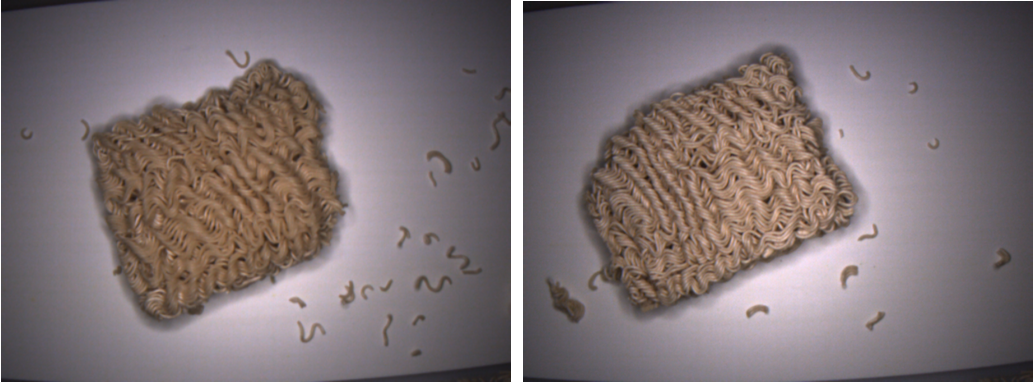
\includegraphics[width=13cm]{assets/PartTwo/Chapterone/DefautNouilles.png}
    \caption{Defaut Nouiiles}
    \label{DefautNouilles1}
    \end{figure}

Nous avons dit précédemment que les réseaux de neurones conventionnels (CNN) sont les plus utilisés pour la détection et la classification des formes et des images. 
Pour cela, notre projet de fin d’étude présenté aborde la problématique de \textbf{\textit{“Quelle est le modèle CNN le plus approprié pour une application de détection de non-conformité ?”}}
\subsection{Hypothèses}  
Suite aux recherches et à l'audition d'experts dans le domaine, les hypothèses suivantes ont été développées : 
\begin{itemize}
    \item Il est préférable d'implémenter un modèle qui avait une architecture dense qui contient plusieurs couches convolutif pour avoir une bonne précision.
    \item Il est préférable d'implémenter un modèle avec un temps d'inférence court pour détecter tous les objets passant sur le convoyeur à grande vitesse.
    \item Il est préférable d'implémenter un modèle de petite taille pour minimiser le temps d’inférence.
\end{itemize}
\newpage
\subsection{Objectif}
Le but de ce travail est de trouver le modèle le plus approprié à utiliser dans une application de détection de non-conformité sur une ligne de production de nouilles. 

Un autre objectif pour nous est de comprendre et d'appliquer les connaissances que nous avons durant notre formation à un scénario du monde réel où nous allons tester notre solution sur un cas réel, tout en utilisant une méthode scientifique. 
\section{Méthodologie du travail}
Du fait de la similarité entre les hypothèses citées ci-dessus, nous avons trouvé intéressant de regrouper les points communs entre ces dernières, qu’ils sont la précision, la taille du modèle et le temps d’inférence. 

En fait, notre travail consiste à identifier un modèle CNN avec un minimum de temps d'inférence, capable de détecter rapidement les nouilles lors de leur passage sur le convoyeur avec une grande vitesse. 

En vue de l’absence de travaux qui traitent un problème de détection similaire au nôtre, nous avons dû définir une démarche spécifique à ce projet. La démarche que nous avons suivie est le fruit de notre réflexion et de notre travail. 
\subsection{Approche}
Pour ce projet, nous avons utilisé une approche comparative qui consiste à évaluer différents modèles de CNN selon des critères précis. Ces critères sont les suivants : 
\begin{itemize}
    \item Le temps d’inférence.
    \item La précision du modèle. 
    \item La taille du modèle. 
\end{itemize}
Nous allons détailler chaque critère ci-dessous : 

\textbf{Le temps d’inférence: }Le temps d'inférence d'un modèle DNN est le temps exécuter par processus de traitement de données pour calculer une sortie telle qu'un score numérique unique. Ce processus est également appelé "mise en production d'un modèle d'apprentissage automatique". 

\textbf{La précision du modèle: }La précision est également appelée valeur prédictive positive. Elle mesure la capacité du modèle à ne pas faire d'erreur lors d'une prédiction positive. La précision est calculée à partir de la matrice de confusion avec la formule suivante : 

\begin{equation}
    P(\%)=\frac{T P+T N}{T P+T N+F P+F N} \times 100
    \end{equation}

Où P désigne la précision et TP, TN, FP, FN sont expliqué dans le chapitre trois de la premiére partie.  
\newpage
\textbf{La taille du modèle :} La taille d'un modèle DNN correspond à la quantité en mégabits (Mb) dont le modèle a besoin pour être stocké dans un environnement approprié .

Le but de ce travail est de trouvé le modèle idéal qui satisfaire les trois caractéristiques. La Figure \ref{ObjectifCible} illustre l’objectif ciblé: 

\begin{figure}[h]
    \centering
    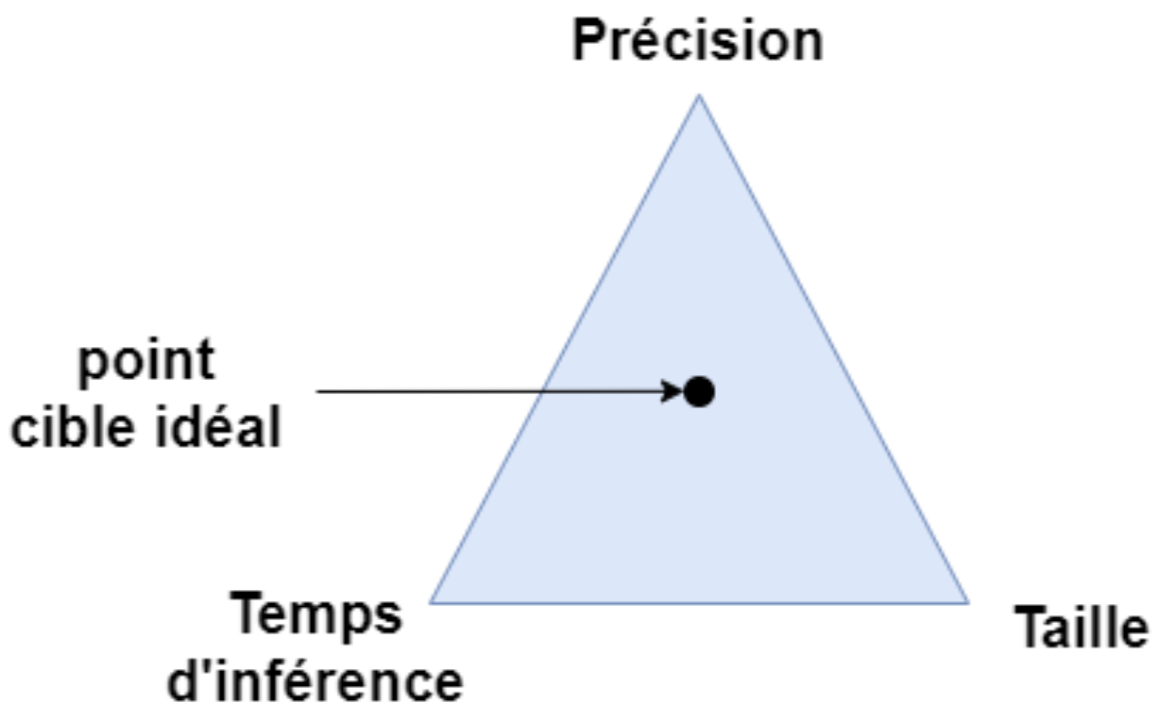
\includegraphics[width=10cm]{assets/PartTwo/Chapterone/ObjectifCible.png}
    \caption{Objectif Cible}
    \label{ObjectifCible}
    \end{figure}

\subsection{Démarche}
Notre approche commence par la collecte des données, qui sont essentiellement des images des nouilles prises par une caméra montée sur la ligne de production. 

La manière de procéder par la suite consiste à : 
\begin{itemize}
    \item Prétraiter les images collectées, afin de mieux exploiter les caractéristiques de ces images. 
    \item Préparer et classer manuellement les images en deux catégories (good / defect) , cette étape est essentielle car nous allons utiliser l'apprentissage supervisé. 
    \item Entraînement des quatre modèles avec les images prétraitées, ces modèles sont sélectionnés à partir d'une évaluation théorique basée sur les spécifications fournies dans la plateforme Keras.
    \item Évaluer chaque modèle de manière pratique sur la base des trois caractéristiques définies dans le point précédent (temps d'inférence, précision et taille du modèle).
    \item Comparer et analyser les trois modèles et sélectionner celui qui convient le mieux à notre solution. 
\end{itemize}
\newpage
Cette démarche peut être visualisée par l’organigramme présent sur la Figure %____%
\newpage
\subsection{Outils}
Plusieurs outils nous ont été utiles dans notre démarche de travail que ce soit en phase d’acquisition, de structuration, de traitement, ainsi que de visualisation des données :
\begin{itemize}
    \item Une caméra est utilisée dans notre solution pour capturer les images des nouilles, c'est une caméra à balayage de zone de marque Mindvision %ref%.
    \item Langage de programmation Python version 3.7. 
    \item La bibliothèque Keras pour utiliser ces modèles CNN.  
    \item Matplotlib pour les graphiques.
    \item Numpy pour les calculs. 
    \item OpenCV pour le traitement d'images. 
    \item Une Edge TPU (NPU) utilisé comme un ordinateur de traitement.
\end{itemize}
\bigskip
\bigskip
D’autres outils nous ont été utiles dans la rédaction du mémoire : 
\begin{itemize}
    \item Google Docs pour la rédaction. 
    \item Draw.io, Adobe Illustrator pour la réalisation des schémas et dessins graphiques. 
    \item Zotero pour la gestion des sources bibliographiques et leur citation.
\end{itemize}

\subsection{Propriété intellectuelle }
Notre travail s'est déroulé au sein d'une entreprise, le code de l'application réalisée et certaines caractéristiques des outils technologiques ne sont donc pas publiables à travers ce document. Certaines données et codes supplémentaires sont présentés en annexe. 

Les schémas et les graphiques sont réalisés par l'auteur, sauf s’ils contiennent une référence ou que le contraire soit explicité. 

\newpage
\section{Conclusion}

Dans ce chapitre, il était question de cadrer notre travail méthodologiquement. Nous avons tout d’abord déterminé les critères à prendre en compte pour notre application qui nous a permis de formuler la problématique et de proposer des hypothèses à vérifier. Par la suite, nous avons présenté notre approche inspirée de la comparaison des modèles CNN pour la classification des images %ref%  
pour traiter notre problématique. 

Enfin, nous avons présenté notre démarche sous la forme d'un organigramme, abordé le point de l'acquisition, du traitement et de la confidentialité des données, et présenté les outils que nous avons utilisés tant pour notre travail que pour ce document.

Dans le prochain chapitre, l'architecture de notre application sera expliquée. De plus, nous allons citer tout le matériel utilisé. Ensuite, on va faire une analyse comparative des modèles CNN existants afin de sélectionner les quatre meilleurs modèles. Enfin, nous allons implémenter et tester chacun de ces quatre modèles afin de sélectionner le meilleur modèle pour notre application. 